\documentclass[]{foi} 
% zakomentirati za pisanje rada na engleskom jeziku
% comment the above line if writing in English

% \documentclass[english]{foi} 
% odkomentirati za pisanje rada na engleskom jeziku
% uncomment the above line if writing in English

\usepackage[utf8]{inputenc}
\usepackage{lipsum}
\usepackage{listings}
\usepackage{color}
\usepackage{xcolor}
\usepackage{minted}



\definecolor{codegreen}{rgb}{0,0.6,0}
\definecolor{codegray}{rgb}{0.5,0.5,0.5}
\definecolor{codepurple}{rgb}{0.58,0,0.82}
\definecolor{backcolour}{rgb}{0.95,0.95,0.92}

\vrstaRada{\projekt}
% \zavrsni ili \diplomski ili \seminar ili \projekt
% type of the paper:
% \seminar is a seminar/term paper
% \projekt is a project

\title{Implementacija Connect Four igre u Pythonu s Minimax Algoritmom}
\predmet{Uvod u umjetnu inteligenciju}
% ostaviti prazno ako \vrstaRada nije \projekt ili \seminar
% \predmetBP ili \predmetDP ili \predmetTBP ili \predmetVAS ili \predmetUUI
% leave it empty if \vrstaRada is not a \projekt or \seminar
% \predmetBP - Databases 1
% \predmetVAS - Multiagent Systems

\author{Ivan Vlašić} 
% ime i prezime studenta/studentice
% name and surname of the author
\spolStudenta{\musko} 
% \zensko ili \musko
% student's gender for grammar purposes: \zensko = F or \musko = M

\mentor{Markus Schatten}
% ime i prezime mentora
% name and surname of the mentor
\spolMentora{\musko} 
% \zensko ili \musko
% mentor's gender: \zensko = F or \musko = M
\titulaProfesora{Prof. dr. sc.}
% HR: dr. sc.  / doc. dr. sc. / izv. prof. dr. sc. / prof. dr. sc. 
% mentor's title:
% EN: -prazno- / Asst. Prof.  / Assoc. Prof.       / Full Prof.

\godina{2024}
\mjesec{Siječanj}
% mjesec obrane rada ili projekta
% year and month of the presentation of the project or paper

\indeks{0016152618}
% broj indeksa ili JMBAG
% author's ID

\smjer{Informacijski i poslovni sustavi}
% (ili:
%     Informacijski sustavi, 
%     Poslovni sustavi, 
%     Ekonomika poduzetništva, 
%     Primjena informacijske tehnologije u poslovanju, 
%     Informacijsko i programsko inženjerstvo, 
%     Baze podataka i baze znanja, 
%     Organizacija poslovnih sustava, 
%     Informatika u obrazovanju
% )
% study programme; please enter "Erasmus" for incoming exchange students


\sazetak{Ovaj rad istražuje implementaciju Connect Four igre koristeći programski jezik Python, s posebnim naglaskom na upotrebu umjetne inteligencije. Teorijsko-metodološko polazište temelji se na analizi algoritma minimax. Kroz projekt, razvijena je simulacija igre s grafičkim sučeljem koristeći pygame biblioteku. Glavne teze rada obuhvaćaju jasnu strukturu koda, praktičnu primjenu minimax algoritma te implementaciju grafičkog sučelja koje poboljšava korisničko iskustvo. Kroz analizu funkcionalnosti poteza igrača i umjetne inteligencije, rad se bavi praktičnom izvedbom igre te naglašava raznolikost poteza umjetne inteligencije. Zaključci ukazuju na uspješnost implementacije, pružajući uvid u primjenu umjetne inteligencije u kontekstu jednostavne igre. Ovaj rad služi kao koristan resurs za razumijevanje umjetne inteligencije u igrama te može poslužiti kao temelj za daljnje istraživanje i edukaciju.}
% abstract of 100 to 300 words.

\kljucneRijeci{Četiri u nizu, Connect four, game, AI}
% keywords including 7 +/- 2 syntagms

\acrodef{VAS}{višeagentni sustav}


\begin{document}

\maketitle

\tableofcontents

\makeatletter \def\@dotsep{4.5} \makeatother
\pagestyle{plain}



\chapter{Uvod}

U današnjem digitalnom dobu, umjetna inteligencija (AI) igra ključnu ulogu u razvoju sofisticiranih sustava s mogućnošću donošenja odluka. Tema ovog seminarskog rada usmjerena je na implementaciju igre s prediktivnim AI protivnikom, posebice korištenjem algoritma minimax. Odabir ove teme proizlazi iz želje za istraživanjem dubljih aspekata umjetne inteligencije kroz prizmu igara, pri čemu će se fokusirati na Connect Four ili na hrvatskom četiri u nizu, popularnu igru koja kombinira strategiju i taktiku.

Motivacija za odabir ove teme leži u želji za razumijevanjem kako algoritmi umjetne inteligencije mogu unaprijediti korisničko iskustvo u igrama te kako se takvi algoritmi mogu prilagoditi različitim scenarijima. Kroz implementaciju Connect Four igre u programskom jeziku Python, očekuje se razvoj AI protivnika koji će koristiti minimax algoritam kako bi pružio izazov igraču.

U glavnom dijelu rada pružit će se definicije ključnih pojmova poput minimax algoritma te teoretski okvir na kojem se temelji opisani formalizam. Osim toga, razmatrat će se praktična izvedivost i primjena predloženog pristupa, istražujući kako se algoritam može prilagoditi dinamici Connect Four igre. 



\chapter{Četiri u nizu ili Connect Four}

Connect Four, poznata i kao "Četiri u nizu" ili "Četiri u liniji", je popularna strategijska igra koja se igra na ploči s 7 stupaca i 6 redaka. Cilj igre je postaviti četiri svoja znaka u nizu, bilo vodoravno, okomito ili dijagonalno, prije suparničkog igrača. Connect Four, ili "Četiri u nizu", je igra koja ima zanimljivu povijest i postala je jedna od najprepoznatljivijih i najigranijih igara na svijetu.  Igra je izvorno patentirana 1974. godine od strane američkog dizajnera Howarda Wexlera i njegovog sina Nila Wexlera. 

Inspiraciju su crpili iz tradicionalnih igara poput "Tic Tac Toa" i "Gomoku". Američka tvrtka za igračke i igre, stekla je prava na igru i proizvodnju, te je od tada distribuirala igru pod svojom popularnom markom "Connect Four". Igra je doživjela mnoge varijacije i digitalne implementacije. Pojavile su se razne verzije s dodatnim značajkama, ali osnovni koncept ostaje nepromijenjen.
Različite varijacije igre su PopOut, Pop10, Five in a row, Power up…

Četiri u nizu se često koristi u školama i obrazovnim ustanovama kao sredstvo za razvoj logičkog razmišljanja i strategijskih vještina kod djece.

Connect Four, poznata i kao 'Četiri u nizu' ili 'Četiri u liniji', nije samo popularna strategijska igra, već je i interesantna u kontekstu umjetne inteligencije. Razmatrano je kako bi se računalima moglo omogućiti izvođenje zadataka za koje ljudi trebaju inteligenciju. Ovo istraživanje reflektira razmišljanje o potencijalima računala i inteligencije, što se može povezati s evolucijom igre 'Connect Four' i njenom adaptacijom kroz godine.

\blockquote[{\cite[str. 5]{allis1988knowledge}}]{One of the first domains in Artificial Intelligence (AI) research, has been computer chess. This
is not surprising, if we consider the possibilities people thought computers would have in the near
future. Using these possibilities, people thought it would be possible to let the computer perform tasks
for which humans need intelligence, whatever that may be.}







\chapter{Pravila i Logika Igre "Connect Four"}

Connect Four je igra koja spaja jednostavnost s dubokom strategijom, pružajući igračima uzbudljivo iskustvo taktičkog razmišljanja. Evo detaljnijeg pregleda pravila i logike igre:

\section{Cilj igre}

Cilj igre je postaviti četiri svoja žetona u nizu, bilo vodoravno, okomito ili dijagonalno, na ploči veličine 7x6. Ova jednostavna pravila čine osnovnu strukturu igre, ali taktički aspekt dodaje dubinu i kompleksnost.

\section{Struktura Ploče}

Igra se odvija na vertikalnoj ploči s 7 stupaca i 6 redaka, ukupno 42 polja. Svaki igrač ima zadatak pametno postavljati svoje žetone na ploču kako bi stvorio pobjednički niz.

\section{Sudionici}

Igra se između dva igrača, pri čemu svaki igrač kontrolira svoje žetone koji su obično različito obojeni. Ova jednostavna podjela stvara osnovu za dinamičan dvoboj između dva igrača.

\section{Potezi}

Igrači naizmjence stavljaju svoje žetone u jedan od sedam stupaca. Žeton zauzima prvo slobodno mjesto na dnu odabranog stupca. Ova slobodna forma postavljanja čini svaki potez važnim, jer igrači moraju odabrati mudro kako bi postigli svoje ciljeve.

\section{Pobjednički Uvjeti}

Pobjednik je igrač koji prvi postavi četiri svoja žetona u nizu, bez obzira na smjer: vodoravno, okomito ili dijagonalno. Ovaj dinamički aspekt povećava potrebu za pažljivim planiranjem svakog poteza.

\section{Neriješeno Stanje}

Ako su svi stupci ispunjeni, a nijedan igrač nije postigao pobjedu, igra završava neriješeno. Ovo dodaje dodatnu tenziju jer igrači moraju balansirati između napada i obrane kako bi izbjegli pat poziciju.

\section{Strategija}

Connect Four zahtijeva duboko taktičko razmišljanje. Igrači moraju simultano blokirati protivničke poteze i graditi vlastitu liniju prema pobjedi. Razvijanje dugoročne strategije i brza prilagodba tijekom igre ključni su za postizanje uspjeha u ovoj dinamičnoj igri. Sposobnost predviđanja poteza protivnika i postavljanje zamki često čine razliku između pobjede i poraza.

Connect Four je dvoslojna igra s potpunim informacijama, suparnička s nul-sumom. Postoje 4,531,985,219,092 mogućih položaja na ploči 7x6.
Ukratko, Connect Four je teorijski riješena igra, gdje prvi igrač može pobijediti uz savršeno igranje.






\chapter{Kritički Osvrt na Implementaciju Connect Four Igre u Pythonu}

U okviru ovog rada, izrađena je simulacija igre Connect Four koristeći programski jezik Python. Ovaj projekt koristi se za istraživanje umjetne inteligencije u kontekstu jednostavne igre.

\section{Korištene Komponente}
\begin{itemize}
    
    \item Numpy: Korišten za manipulaciju višedimenzionalnim poljima, posebno za stvaranje i upravljanje igraćom pločom.
    \item Pygame: Grafička biblioteka koja omogućuje vizualno sučelje igre, čineći je pristupačnom i zabavnom.
    \item Math: Korišten za osnovne matematičke operacije potrebne tijekom izvođenja igre.
\end{itemize}
\section{Algoritam}
\begin{itemize}
    \item Minimax: Ključni dio implementacije za odlučivanje poteza umjetne inteligencije. Minimax pristup omogućuje sustavno ocjenjivanje svih mogućih poteza. ovaj algoritam se primjenjuje u igrama gdje postoji dvoje igrača koji se izmjenjuju u odabiru poteza, a broj mogućih poteza za određenu poziciju u igri je unaprijed poznat.


 \blockquote[{\cite[str. 2]{borovska2007efficiency}}]{Minimax algorithm can be applied providing there are two players in the game who
take turns at playing with a given number of possible moves for a given position in the
game. The game is determined, i.e. the game does not employ dice rules of moves. The
game is characterized by information transparency, i.e. each player knows the whole state
of the game at each position. The leaves of the game tree present the final game positions
where the outcome of the game is obvious. The aim of the minimax search in the game
tree is to find the optimal strategy as a sequence of best possible moves of a given player
taking into account possible moves of the other player up to a given depth.}

\end{itemize}
\section{Praktična Izvedivost}
\begin{itemize}
    \item Jednostavnost Implementacije: Kod je jasno strukturiran i pristupačan, što olakšava razumijevanje i eventualne modifikacije.
    \item Grafičko Sučelje: Korištenjem pygame-a, implementirano je grafičko sučelje koje olakšava praćenje tijeka igre.
    \item Funkcionalnost Poteza: Potezi igrača i umjetne inteligencije su implementirani prema pravilima igre, uz primjenu minimax algoritma za dinamičko odlučivanje umjetne inteligencije.
\end{itemize}
\section{Primjena}
\begin{itemize}
    \item Razvoj Umjetne Inteligencije: Projekt pruža primjer primjene umjetne inteligencije u jednostavnom igraćem okruženju, koristeći minimax algoritam.
\end{itemize}






\chapter{Programski kod}

Riješenje igre koju igramo protiv AI u python-u napisan je ispod te se nalazi i opis implementacije.



\begin{listing}
    \begin{minted}{python}
import random
import sys
import numpy as np
import math
import pygame
def postavi_parametre():
    global ljubicasta,tamno_plava, Red,Stupac,duzina_niza,roza,UmjetnaInt_zeton, Prazno, covjek_zeton,narancasta, tamno_zelena, bijela
    ljubicasta =(128, 0, 1285)
    tamno_plava= (0, 0, 139)
    Red=6
    Stupac =7
    duzina_niza = 4
    roza =(255, 192, 203)
    UmjetnaInt_zeton= 2
    Prazno =0
    covjek_zeton =1
    narancasta=(255, 165, 0)
    tamno_zelena=(0, 128, 0)
    bijela=(255, 255, 255)

postavi_parametre()


def procjeni(rupa, zeton): 
    zgoditak= 0
    opp_zeton= UmjetnaInt_zeton if zeton == covjek_zeton else covjek_zeton
    if rupa.count(zeton) == 4:
        zgoditak += 200
    elif rupa.count(zeton)==3 and rupa.count(Prazno)== 1:
        zgoditak += 10
    elif rupa.count(zeton)== 2 and rupa.count(Prazno) ==2:
        zgoditak += 4
    if rupa.count(opp_zeton)==3 and rupa.count(Prazno) ==1:
        zgoditak -= 8

    return zgoditak
    \end{minted}
    \caption{Isječak koda}
    \label{lst:dva}
\end{listing}

\begin{listing}
    \begin{minted}{python}
def procjeni_poziciju(ploca, zeton):
    

    ## zgoditak center stupacumn
    srednje_brojanje= np.count_nonzero(ploca[:, Stupac // 2]== zeton)
    zgoditak=0
    zgoditak += srednje_brojanje * 3

    ##Horizontalo
    r = 0
    while r<Red:
        red_polja= [int(i) for i in list(ploca[r, :])]
        c= 0
        while c< Stupac - 3:
            rupa= red_polja[c:c + duzina_niza]
            zgoditak += procjeni(rupa, zeton)
            c += 1
        r += 1

    ##Vertikalno
    c= 0
    while c <Stupac:
        stupac_polja =[int(i) for i in list(ploca[:, c])]
        r =0
        while r < Red -3:
            rupa = stupac_polja[r:r + duzina_niza]
            zgoditak +=procjeni(rupa, zeton)
            r +=1
        c +=1

    ##dijagonalu prema gore
    r =0
    while r<Red -3:
        c= 0
        while c < Stupac - 3:
            rupa = [ploca[r + i][c + i] for i in range(duzina_niza)]
            zgoditak += procjeni(rupa, zeton)
            c +=1
        r+=1

    ##dijagonalu prema gore
    r=0
    while r< Red -3:
        c =0
        while c< Stupac -3:
            rupa = [ploca[r+3- i][c+i] for i in range(duzina_niza)]
            zgoditak+= procjeni(rupa, zeton)
            c+= 1
        r +=1

    return zgoditak
    \end{minted}
    \caption{Isječak koda}
    \label{lst:dva}
\end{listing}

\begin{listing}
    \begin{minted}{python}
def postavi_na_vrh(ploca, stupac):
    r=0
    while r <Red:
        if ploca[r][stupac] == 0:
            return r
        r +=1


def pobjednicki_potez(ploca, zeton):
    #horizontalo
    c =0
    while c < Stupac - 3:
        r = 0
        while r < Red:
            if ploca[r][c + 1] == zeton and ploca[r][c] == zeton:
                if ploca[r][c + 2] == zeton and ploca[r][c + 3] == zeton:
                    return True
            r += 1
        c += 1

    #vertikalno
    c = 0
    while c < Stupac:
        r = 0
        while r < Red - 3:
            if ploca[r][c]== zeton and ploca[r + 1][c] == zeton:
                if ploca[r+ 2][c] ==zeton and ploca[r +3][c]== zeton:
                    return True
            r += 1
        c += 1

    #diagnoalno gore
    c = 0
    while c <Stupac -3:
        r =0
        while r < Red -3:
            if ploca[r][c]== zeton and ploca[r +1][c +1] == zeton:
                if ploca[r + 2][c + 2] == zeton and ploca[r +3][c +3] == zeton:
                    return True
            r +=1
        c +=1

    # diagonalno dolje
    c =0
    while c < Stupac -3:
        r =3
        while r <Red:
            if ploca[r][c] == zeton and ploca[r - 1][c + 1] == zeton:
                if ploca[r - 2][c + 2] ==zeton and ploca[r -3][c +3] == zeton:
                    return True
            r +=1
        c +=1

    return False
    \end{minted}
    \caption{Isječak koda}
    \label{lst:dva}
\end{listing}


\begin{listing}
    \begin{minted}{python}
def terminal_node(ploca):
    return pobjednicki_potez(ploca, covjek_zeton) or pobjednicki_potez(ploca, UmjetnaInt_zeton) or len(get_odobrena_lokacija(ploca)) == 0



def polje_postavljanja(ploca, red, stupac, zeton):
    ploca[red][stupac] =zeton

    \end{minted}
    \caption{Isječak koda}
    \label{lst:dva}
\end{listing}

\begin{listing}
    \begin{minted}{python}
def minimax(ploca, dubina, a, b, igracc):
    
    def zadavanje_vrijednsoti(stupac, new_zgoditak):
        nonlocal vrijednost
        nonlocal stupacumn
        vrijednost =new_zgoditak
        stupacumn =stupac
        
    
    terminal =terminal_node(ploca)
    odobrena_lokacija =get_odobrena_lokacija(ploca)
  
    if terminal or dubina ==0:
        return (
            (None, 1000000000) if pobjednicki_potez(ploca, UmjetnaInt_zeton)
            else (None, -100000000) if pobjednicki_potez(ploca, covjek_zeton)
            else (None, procjeni_poziciju(ploca, UmjetnaInt_zeton)) if dubina == 0
            else (None, 0)
        )

    
    if igracc:
        vrijednost= -math.inf
        stupacumn= random.choice(odobrena_lokacija)
    else:
        vrijednost =math.inf
        stupacumn =random.choice(odobrena_lokacija)
        
    for stupac in odobrena_lokacija:
            
        red= postavi_na_vrh(ploca, stupac)
        B= ploca.copy()
        if igracc:
            polje_postavljanja(B, red, stupac, UmjetnaInt_zeton)
        else:
            polje_postavljanja(B, red, stupac, covjek_zeton)
        if igracc:
            new_zgoditak= minimax(B, dubina - 1, a, b, False)[1]
            if new_zgoditak > vrijednost:
                zadavanje_vrijednsoti(stupac, new_zgoditak)
        else:
            new_zgoditak = minimax(B, dubina - 1, a, b, True)[1]
            if new_zgoditak < vrijednost:
                zadavanje_vrijednsoti(stupac, new_zgoditak)
       
        if igracc:
            a= max(a, vrijednost)
        else: 
            b= min(b, vrijednost)

        if a >= b:
            break
    return stupacumn, vrijednost
    \end{minted}
    \caption{Isječak koda}
    \label{lst:dva}
\end{listing}

\begin{listing}
    \begin{minted}{python}
def provjera_polja(ploca, stupac):
    return ploca[Red -1][stupac] == 0

def get_odobrena_lokacija(ploca):
    return [stupac for stupac in range(Stupac) if provjera_polja(ploca, stupac)]


def dizajn_ploce(ploca):
    c =0
    while c < Stupac:
        r =0
        while r < Red:
            pygame.draw.rect(sucelje, bijela, (c * dimenzije, r * dimenzije + dimenzije, dimenzije, dimenzije))
            pygame.draw.circle(sucelje, tamno_plava, (c * dimenzije + dimenzije // 2, r * dimenzije + 3 * dimenzije // 2), RADIUS)
            r +=1
        c +=1

    c =0
    
    while c < Stupac:
        r= 0
        while r < Red:
            if ploca[r][c] == covjek_zeton:
                pygame.draw.circle(sucelje, narancasta, (c * dimenzije + dimenzije // 2, height - r * dimenzije - dimenzije // 2), RADIUS)
            elif ploca[r][c] == UmjetnaInt_zeton:
                pygame.draw.circle(sucelje, roza, (c * dimenzije + dimenzije // 2, height - r * dimenzije - dimenzije // 2), RADIUS)
            r +=1
        c +=1

    pygame.display.update()

def postavi_sučelje(dimenzije):
    global RADIUS ,sucelje, myfont
    RADIUS = int(dimenzije / 2-2)
    sucelje = pygame.display.set_mode(size)
    myfont = pygame.font.SysFont("monospace", 45)
    \end{minted}
    \caption{Isječak koda}
    \label{lst:dva}
\end{listing}

\begin{listing}
    \begin{minted}{python}
def polje_igranja():
    ploca =np.zeros((Red, Stupac))
    return ploca


def print_ploca(ploca):
    print(np.flip(ploca, 0))

ploca =polje_igranja()
print_ploca(ploca)
game_over= False

pygame.init()
dimenzije =89

width, height = Stupac *dimenzije, (Red + 1) *dimenzije
size = (width, height)
postavi_sučelje(dimenzije)
covjek =0
UmjetnaInt =1

dizajn_ploce(ploca)
pygame.display.update()

turn = random.randint(covjek, UmjetnaInt)
    \end{minted}
    \caption{Isječak koda}
    \label{lst:dva}
\end{listing}

\begin{listing}
    \begin{minted}{python}
while not game_over:
    
    def update_game_state():
        global turn
        turn += 1
        turn %= 2
        print_ploca(ploca)
        dizajn_ploce(ploca)

     
    for event in pygame.event.get():
        if event.type == pygame.QUIT:
            pygame.quit()
            sys.exit()

        if event.type == pygame.MOUSEMOTION or (turn == covjek and event.type == pygame.MOUSEBUTTONDOWN):
            pygame.draw.rect(sucelje, tamno_zelena, (0, 0, width, dimenzije))
            pygame.display.update()

            if turn == covjek and event.type == pygame.MOUSEBUTTONDOWN:
                posx = event.pos[0]
                stupac = posx // dimenzije

                if provjera_polja(ploca, stupac):
                    red = postavi_na_vrh(ploca, stupac)
                    polje_postavljanja(ploca, red, stupac, covjek_zeton)

                    if pobjednicki_potez(ploca, covjek_zeton):
                        sucelje.blit(myfont.render("Pobjedio s!!!!!!!!", 1, narancasta), (40, 10))
                        game_over = True

                    update_game_state()


    if turn == UmjetnaInt and not game_over:
        stupac, minimax_zgoditak =minimax(ploca, 5, -math.inf, math.inf, True)

        if provjera_polja(ploca, stupac):
            red = postavi_na_vrh(ploca, stupac)
            polje_postavljanja(ploca, red, stupac, UmjetnaInt_zeton)

            if pobjednicki_potez(ploca, UmjetnaInt_zeton):
                sucelje.blit(myfont.render("Pobjedio je AI !!!!!!!!", 1, narancasta), (40, 10))
                game_over =True

            update_game_state()


    if game_over:
        pygame.time.wait(5000)
    
    \end{minted}
    \caption{Isječak koda}
    \label{lst:dva}
\end{listing}


\chapter{Objašnjenje koda}

\section{Bibilioteke i moduli}
Na početku koda su navedeni određeni moduli i biblioteke koje koristi program.
\begin{enumerate}
    \item \texttt{random}: Koristi se za generiranje nasumičnih brojeva.
    \item \texttt{sys}: Omogućuje pristup funkcionalnostima povezanim sa sustavom.
    \item \texttt{numpy (np)}: Koristi se za rad s višedimenzionalnim poljima.
    \item \texttt{math}: Koristi se za korištenje matematičkih funkcija.
    \item \texttt{pygame}: Biblioteka za izradu igara i grafičkih korisničkih sučelja.
\end{enumerate}

\section{Funkcije}

\subsection{Organizacija funkcija}
S ciljem poboljšanja čitljivosti i održivosti implementacije igre "Connect Four", kod je logički organiziran u dvije glavne sekcije: \textbf{Funkcije Grafičkog Sučelja}, \textbf{Logika Igre} i \textbf{Parametri}.

\subsubsection{Funkcije Grafičkog Sučelja}

Funkcije Grafičkog Sučelja obuhvaćaju kod odgovoran za grafičko korisničko sučelje (GUI) igre "Connect Four". Ove funkcije rješavaju prikaz igre, igračkih žetona i interakcija s korisnikom. Glavni cilj ove sekcije je osigurati vizualno privlačno i korisnički prihvatljivo iskustvo igranja.

\begin{itemize}
    \item \texttt{dizajn\_ploce}: Crtanje vizualnog prikaza ploče igre pomoću Pygame biblioteke, uključujući boje i položaje žetona.
    \item \texttt{postavi\_sučelje}: Postavljanje sučelja igre pomoću Pygame-a, uključujući dimenzije prozora i font koji se koristi za prikazivanje poruka tijekom igre.
    \item \texttt{polje\_igranja}: Inicijalizacija igre, postavljanje početne ploče i drugih parametara potrebnih za igru.
    \item \texttt{print\_ploca}:  Ispis trenutnog stanja ploče u konzoli. Koristi se uglavnom u svrhu debagiranja.
    \item \texttt{update\_game\_state}: Ažuriranje stanja igre nakon svakog poteza, uključujući provjeru pobjednika, ažuriranje vizualnog prikaza i promjenu redoslijeda igrača.
    \item \texttt{zadavanje\_vrijednosti}: Pomoćna funkcija koja postavlja vrijednost i stupac na temelju zadane vrijednosti. Koristi se unutar minimax algoritma.
\end{itemize}

\subsubsection{Logika igre}

Funkcije Igre obuhvaćaju osnovnu logiku igre "Connect Four". Ove funkcije bave se aspektima kao što su evaluacija poteza, određivanje pobjednika i izvođenje optimalnih poteza umjetne inteligencije (AI). Glavni cilj ove sekcije je implementirati osnovna pravila i mehanike igre.

\begin{itemize}
    \item \texttt{procjeni}: Ova funkcija ocjenjuje trenutno stanje niza na ploči dodjeljujući bodove prema određenim pravilima. Na primjer, dodaju se bodovi za redove, stupce ili dijagonale s više žetona istog igrača.
    \item \texttt{procjeni\_poziciju}: Sumira zgoditke za određenu poziciju na ploči, uzimajući u obzir horizontalne, vertikalne i dijagonalne linije. Koristi se kako bi se odredila vrijednost određene pozicije tijekom izvođenja minimax algoritma.
    \item \texttt{postavi\_na\_vrh}: Pronalazi prvo slobodno mjesto na odabranom stupcu i postavlja žeton igrača na vrh tog mjesta. Ova funkcija je ključna za implementaciju poteza igrača.
    \item \texttt{pobjednicki\_potez}: Ova funkcija provjerava je li trenutni potez pobjednički, odnosno je li igrač postigao niz od četiri žetona u bilo kojem smjeru - vodoravno, vertikalno ili dijagonalno.
    \item \texttt{terminal\_node}:  Provjerava je li trenutno stanje ploče terminalno, odnosno je li igra gotova jer je jedan od igrača pobijedio ili nema više slobodnih mjesta za poteze.
    \item \texttt{polje\_postavljanja}: Postavlja žeton na određeno mjesto na ploči, a koristi se nakon što se odabere stupac za potez.
    \item \texttt{minimax}: Ovo je implementacija minimax algoritma koji se koristi za izračun optimalnog poteza umjetne inteligencije. Algoritam traži najbolji potez koji minimizira ili maksimizira vrijednost ovisno o tome je li trenutni potez za umjetnu inteligenciju ili igrača.
\end{itemize}

\subsubsection{Parametri}
\begin{itemize}
    \item \texttt{postavi\_parametre}: Ova funkcija postavlja globalne parametre igre kao što su boje, broj redova i stupaca, duljina niza za pobjedu te druge vrijednosti koje će se koristiti tijekom izvođenja igre..
\end{itemize}
Ove jasno odvojene sekcije doprinose modularnosti i razumljivosti koda, čineći ga lakšim za održavanje, otklanjanje pogrešaka i proširenje igre "Connect Four".


\subsubsection{Minimax algoritam}


\textbf{Inicijalizacija Terminalnog Čvora (\texttt{terminal\_node}):}
Funkcija \texttt{terminal\_node} provjerava je li trenutno stanje igre terminalno, odnosno je li došlo do pobjede nekog igrača ili je ploča popunjena. Vraća \texttt{True} ako je igra završena, inače \texttt{False}.

\textbf{Odobrena Lokacija (\texttt{get\_odobrena\_lokacija}):}
Funkcija \texttt{get\_odobrena\_lokacija} vraća listu stupaca na kojima se može postaviti žeton, tj. stupce koji nisu potpuno popunjeni.

\textbf{Procjena Pozicije (\texttt{procjeni\_poziciju}):}
Funkcija \texttt{procjeni\_poziciju} ocjenjuje trenutno stanje igre za određenog igrača. Prati zgoditke na horizontali, vertikali i dijagonalama, dodjeljujući ocjene ovisno o prisutnosti određenih uzoraka.

\textbf{Postavljanje Žetona na Vrh (\texttt{postavi\_na\_vrh}):}
Funkcija \texttt{postavi\_na\_vrh} pronalazi prvi slobodan redak u odabranom stupcu i postavlja žeton tog igrača.

\textbf{Pobjednički Potez (\texttt{pobjednicki\_potez}):}
Funkcija \texttt{pobjednicki\_potez} provjerava je li trenutno postavljeni žeton rezultirao pobjedom (četiri u nizu) na horizontali, vertikali ili dijagonalama.

\textbf{Zadavanje Vrijednosti (\texttt{zadavanje\_vrijednosti}):}
Unutarnja funkcija \texttt{zadavanje\_vrijednosti} služi za postavljanje nove vrijednosti i odgovarajućeg stupca u slučaju da se pronađe bolji potez tijekom pretrage.

\textbf{Minimax Algoritam (\texttt{minimax}):}
Glavna funkcija \texttt{minimax} implementira minimax algoritam. Rekurzivno istražuje stablo igre, odabire najbolji potez za umjetnu inteligenciju i vraća odgovarajući stupac i pripadajuću vrijednost.


\subsection{Glavna Petlja Igre}

Glavna petlja igre se izvršava sve dok igra nije završena. Unutar petlje se obrađuju događaji, ažurira stanje igre i provjeravaju potezi igrača i umjetne inteligencije.

\textbf{Provjera Događaja:}
\begin{itemize}
    \item Ako korisnik zatvori prozor, igra se završava.
    \item Ako je red na potezu čovjek i klikne na ekran, igra reagira na odabir stupca i postavlja žeton.
\end{itemize}

\textbf{Potez Umjetne Inteligencije (AI):}
\begin{itemize}
    \item Ako je red na potezu umjetna inteligencija, koristi se algoritam minimax za odabir najboljeg poteza.
\end{itemize}

\textbf{Ažuriranje Stanja Igre:}
\begin{itemize}
    \item Ažurira se red na potezu, prikazuje trenutno stanje ploče i osvježava sučelje igre.
\end{itemize}

\textbf{Završetak Igre:}
\begin{itemize}
    \item Ako je igra završena, program čeka 3 sekunde prije zatvaranja prozora pygame.
\end{itemize}

Ova petlja osigurava nesmetan tijek igre, interakciju s korisnikom i poteze umjetne inteligencije.


\chapter{Prikaz rada aplikacije}

U ovom dijeli rada ćemo prikazati u par slika rad aplikacije.

\begin{figure}[]
    \centering
    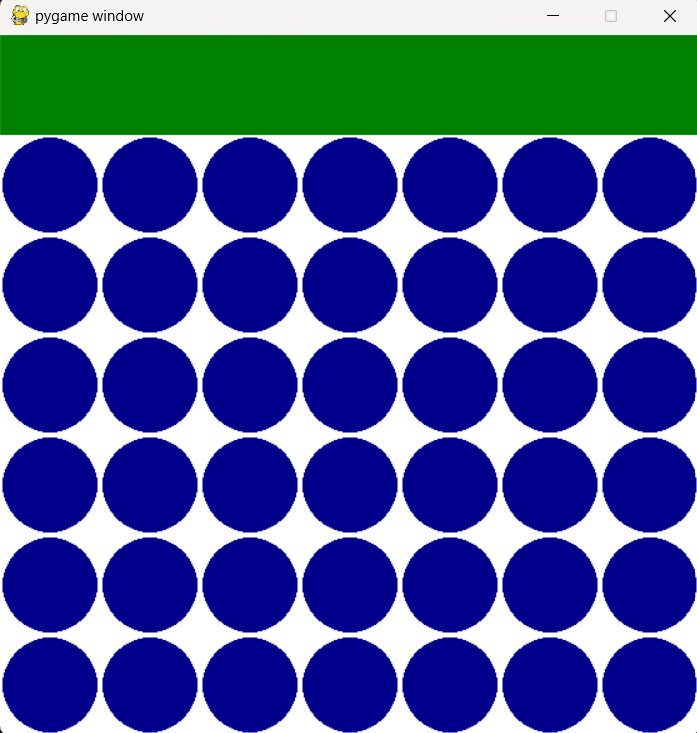
\includegraphics[width=0.9\textwidth]{slike/1.png}
    \caption{Prvi potez je imao igrač te zatim odmah AI radi svoj potez}
    \label{Slika1}
\end{figure}

\begin{figure}[]
    \centering
    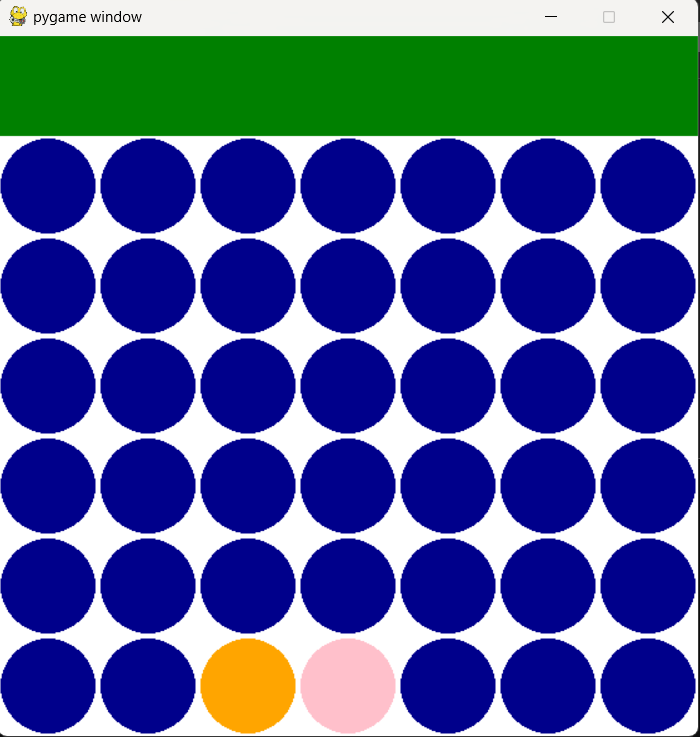
\includegraphics[width=0.9\textwidth]{slike/2.png}
    \caption{drugi potez je napravio igrač te zatim odmah AI radi svoj potez}
    \label{Slika1}
\end{figure}

\begin{figure}[]
    \centering
    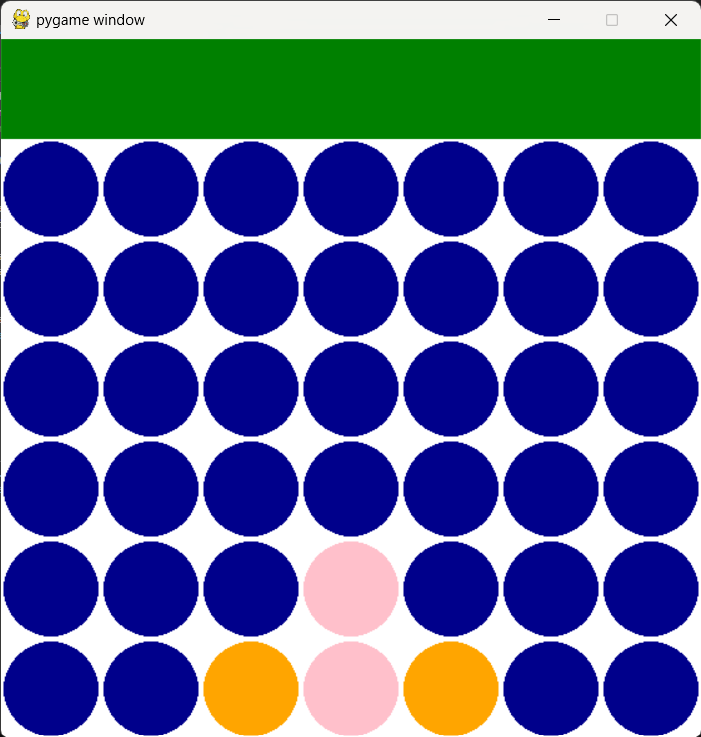
\includegraphics[width=0.9\textwidth]{slike/3.png}
    \caption{Nakon 3 poteza igrača AI radi svoj potez}
    \label{Slika1}
\end{figure}

\begin{figure}[]
    \centering
    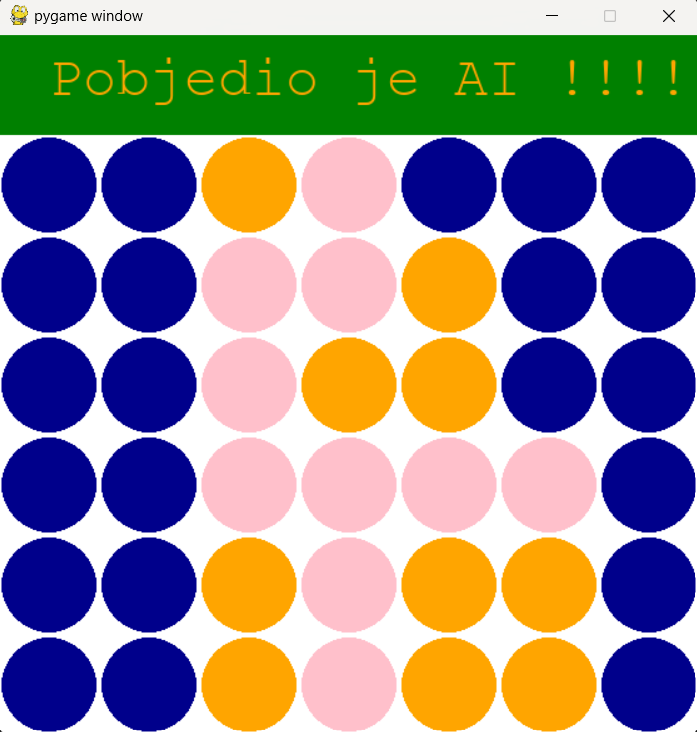
\includegraphics[width=0.9\textwidth]{slike/4.png}
    \caption{Nakon par poteza igrača AI radi svoj potez i pobjeđuje}
    \label{Slika1}
\end{figure}

\chapter{Zaključak}

U ovom istraživačkom radu istražena je implementacija Connect Four igre s naglaskom na upotrebu umjetne inteligencije. Kroz analizu algoritma minimax, razvijena je simulacija igre koristeći programski jezik Python, uz primjenu pygame biblioteke za grafičko sučelje. Glavne teze rada obuhvaćaju jasnu strukturu koda, praktičnu primjenu minimax algoritma te implementaciju grafičkog sučelja radi poboljšanja korisničkog iskustva.

Rad se fokusira na ključna pravila i logiku igre Connect Four, gdje igrači ciljaju postavljanje četiri svoja žetona u nizu, bilo vodoravno, okomito ili dijagonalno. Prikazane su strategije igre, uključujući potrebu za taktičkim razmišljanjem, blokiranjem protivničkih poteza te razvojem dugoročne strategije.

Kroz kritički osvrt na implementaciju u Pythonu, rad prepoznaje važnost korištenja algoritma minimax s Alpha-Beta podrezivanjem za odlučivanje poteza umjetne inteligencije. Navedene su korištene komponente poput NumPy-a i Pygame-a te istaknuta je praktična izvedivost projekta, uz jednostavnu implementaciju, jasnu strukturu koda te grafičko sučelje koje olakšava praćenje tijeka igre.

Zaključci ukazuju na uspješnost implementacije i pružaju uvid u primjenu umjetne inteligencije u kontekstu jednostavne igre poput Connect Four. Rad se smatra korisnim resursom za razumijevanje umjetne inteligencije u igrama te može poslužiti kao temelj za daljnje istraživanje i edukaciju u području AI.



\makebackmatter

\nocite{pygame,Geeksforgeeks,TheSharperDev,techwithtim,OpenAI}





\end{document}
